\chapter{PHP to .NET compilation}
The third chapter talks about programming languages and communities around them in general. It provides a possible way of building a bridge between two selected communities and outlines some aspects of its practical implementation. Peachpie, an actual implementation of previously discussed tool is presented.

\section{Motivation}
In the recent days, web development, and software development in general, has evolved by a great bit in both the number of people involved and in a size of code produced. Web pages and applications are no longer just a several thousands of lines of code. For instance Facebook, one of the most profound social networks in the world, has a codebase of over 50 millions of lines of code \citep{Knowledge}. Moreover, it's not unusual for a codebase of software of an average modern high-end car to reach a hundred million lines of code \citep{Knowledge}. 

Natural consequence of such technological growth is that it is no longer possible to develop complex software alone and almost everything requires teaming up. Above the project-related groups of developers stands a community, where knowledge is shared and people learn from each other. While some patterns and practices are applicable in general, with increasing complexity of problem their amount is smaller and their usefulness decreases. This need for more definite knowledge has caused the community to be rather granulated and the number of breaching criteria is immense. Undoubtedly the most commonly used criteria is the one of programming languages.

A reasonable effort is put into attempts to bring together selected language-level sub-communities. Going through all of the possible methods of achieving this, is beyond the scope of the theses, so we will simply pick the one that is further relevant, the compilation method. It is worth mentioning that for this compilation method we require the target language to be an interpreted language. It is not to be misunderstood with method of compiling the second language to the source code of the target language, which would in that case be called the transcompilation method. Simply speaking, our compilation method means that we have a language A compiling into an interpreted language that is later executed. Then we take a language B and compile it with special tool into the same intermediate language as the language A. This allows us to embed parts of code from language B within our application written in language A. When this approach does not literally merge the sub-communities of languages A and B, it clearly provides a bridge between the two in a way of using features, knowledge and finally the developers of both languages in a single project \citep{Peachpie}.

For later usage, we would require a target language to be a compiled language with an efficient way to execute compiled code separated into multiple files. As was mentioned before, C\# is a compiled language with strictly defined foundation \citep{microsoft.docs}. In addition to, it has quite intuitive Integrated Development Environment (IDE) provided by Microsoft Corporation with many built-in features such as profiler and web designer \citep{microsoft.docs}. Finally, its assembly system allows for splitting application code between multiple files and their later efficient combination on runtime. For these reasons it is a perfect target for a compilation. On the other hand, PHP is an interpreted language with a large community of developers, many implemented libraries and vastly popular frameworks. Making it a possible candidate for a compilation.




\section{Languages comparison}
In programming generally, it is fairly unusual for two programming languages to share all, the same philosophy, capabilities and area of usage. When a problem in a certain language is encountered, solutions in other languages are mostly useless. This is addressed by a compilation method introduced before. When we encounter a problem in one language, have the solution in another language and ultimately have the means of compiling one language to another, the former solution quickly comes in hand. The crucial spot in the process are mentioned means for achieving the compilation. Prior to learning how to operate with the compiler tool, we first need to compare our candidates for the source and the target language. That is necessary in order to prepare for possible complications that might occur during the actual compilation.


\paragraph{Type System}
Even though there are significant differences in languages' type systems - one is statically typed, where the other one is dynamically typed, this difference will introduce no noticeable difficulties. PHP's engine is using types internally and those basic types are subset of the CTS \citep{php.internals, Ecma335}. In addition to, PHP has no sense of topology in its type system \citep{php.manual}. The types simply exist without any base types or inherited functions \citep{php.manual}. This makes their mapping to the .NET types and into its type hierarchy rather easy.

The only type-related complication is PHP's implicit conversion between the types. However, this problem can be solved easily by adding explicit conversions, implementing special functions that emulate PHP's implicit conversions between the types or for the sake of expensiveness using base type \texttt{Object} \citep{Phalanger}.


\paragraph{Variables}
As we already know, PHP does require type-less variable initialization whereas C\# requires explicit type definition when a new variable is initialized. Furthermore, PHP needs no variable initialization at all. On the contrary, C\#  presents a rule for each variable usage called the definitive assignment.

The problem of PHP's type-less initialization can be easily solved using implicit conversions mentioned in preceding paragraph and C\#'s base class \texttt{Object} \citep{Phalanger}. The problem of definitive assignment and PHP's ability to define variables in-place can be addressed on compilation \citep{Peachpie}. Based on each variable's usage, and for the sake of definitive assignment it can be simply initialized to null if needed. This operation will satisfy C\#'s variable requirements and will not divert from the behaviour observed in PHP, where uninitialized variables return null upon reading.


\paragraph{Execution}
One of the main differences between C\# and PHP lays in their execution. PHP is interpreted language whereas C\# is compiled. Although this difference in a deployment process might seem problematic, it is actually in our favour. If we were attempting to compile C\# to PHP, this might not be true as regarding PHP application's execution, such process would require compiler to transform C\# code to native PHP code.

On the other hand, in out case, we want to compile code of interpreted language to a code of compiled language. Although converting PHP code directly to C\# code is also a solution, it is rather poor one as there would be two compilations in a process of deploying such application which would bring significant overhead.

Solution to this is .NET, more specifically the CLI. If we can compile PHP code into C\# code that can be later compiled into managed code, by the law of transitivity, we have to be able to compile PHP code into managed code directly \citep{Phalanger}. The comparison of languages' deployment extended by the provided solution is depicted in the Figure 3.1.

\begin{figure}[h!]
  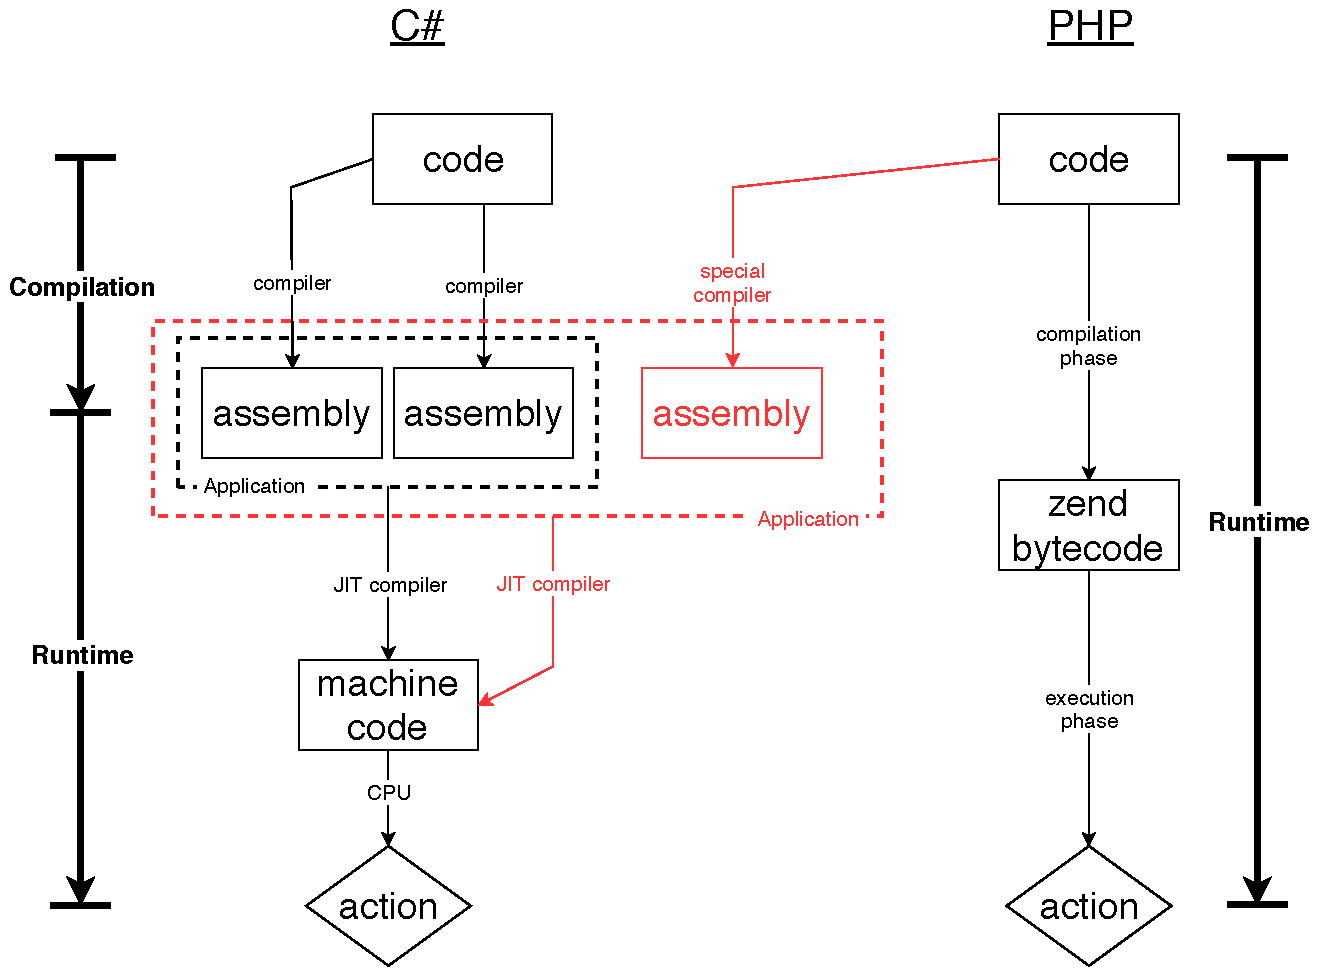
\includegraphics[width=\linewidth]{img/PHP_to_Csharp.pdf}
  \caption{PHP to C\# deployment comparison}
  \label{fig:php_csharp_comparison}
\end{figure}


\paragraph{Consequences}
The first consequence originates from the way PHP is executed. Because everything in PHP is done on runtime, parts of the code may, and sometimes do, contain by a program flow non-accessible invalid code, that would cause PHP's interpreter to throw runtime exception when executed. It is obvious that such feature cannot be brought to the world of .NET because of the compilation that validates the code in the process. For such code, there is no other way than to either remove it from the source, or exclude the whole file from the application.

The second consequence does not originate from anything mentioned but is more of an architectural nature. CLR does require whole \texttt{finally} block to be executed and for this purpose forbids statements redirecting the execution flow elsewhere \citep{microsoft.docs}. On the other hand, PHP guarantees only \texttt{finally} block entering, not its whole execution, allowing it to contain flow control statement such as \texttt{return}, which will result in overwriting the possible \texttt{try/catch} block return value \citep{php.manual}. Again, as such behaviour is inconsistent, there is no other way than to either rewrite these statements to an equivalent form without unsupported constructs, or to exclude them if the former is not possible.

Very similar differences can be observed in iterators as well. Where C\# does place further restrictions on usage of \texttt{yield} keyword in combination with \texttt{try, catch} and \texttt{finally} blocks, PHP does not \citep{microsoft.docs, php.manual}. This diversity originates again in the language-specific procession of exception handling blocks and its possible solutions are for this reason same to the preceding paragraph. 

Last but not least stands the problem of standardization. Because PHP language does not have any complete formal standard, there is no list of all defined functions, classes and possible parameters. This makes it almost impossible task to create a compiler tool which would be able to process every PHP's built in function, because that would require having cumulative knowledge of all of these. For this reason, it is beyond the capabilities of a few individuals who usually work together on such compiler and so they have to be always prepared for further compiler enhancing and additional features implementing.



\section{Peachpie}
After theoretical analysis of the languages, providing a brief outline of possible complication that might arise during compilation and presenting some of possible solutions for each of them, we can finally proceed to the actual compiler tool, Peachpie.

Peachpie is a modern PHP compiler based on Roslyn, a set of open-source compilers and code analysis APIs, also called .NET compiler platform \citep{Peachpie, microsoft.docs}. Peachpie took heavy inspiration in its predecessor Phalanger, a PHP language compiler for .NET Framework targeting the PHP language version 5 and ASP.NET 2.0 \citep{Peachpie, Phalanger}. Peachpie allows for a full compatibility with .NET, which enables the development of hybrid applications, where part of the code is written in C\# and part in PHP \citep{Peachpie}. Finally, Peachpie allows for PHP applications to be developed directly in Microsoft Visual Studio IDE \citep{Peachpie}. This way, developers can make full use of its built in features such as profiling or debugging.

\paragraph{Development}
When Phalanger was developed, its main goal was to compile legacy PHP code into .NET, at which it ultimately succeeded. However, its development slowed down through out the time and finally stopped at PHP language version 5.6 \citep{Peachpie}. 

Several years later, Microsoft introduced compiler platform called Roslyn \citep{Peachpie}. Aside from granting tools to potentially speed up both compilation and runtime phase, it also provides a way to help developers directly perform phases of compilation, such as lexical and syntactic analysis \citep{Peachpie}. Inspired by the Roslyn platform, former maintainers of Phalanger revived the concept of PHP compiler for .NET and Peachpie's development was initiated \citep{Peachpie}. 

The compiler's development continues to the present day and new development versions of software are released several times a month, each time bringing additional functionalities and missing features implementation \citep{peachpie.github}. At the time of writing, Peachpie is capable of compiling PHP versions 5.4 up to 7.4, using it within .NET Core SDK 2.1 or newer and is compatible with .NET Core 3.1 as well\citep{Peachpie, peachpie.github}.


\paragraph{Benefits of Peachpie}
Comparing and benchmarking speed of Peachpie and PHP is rather complicated task and to achieve certain reliability, it would require to perform several tightly designed tests across multiple platforms and on a wide variety of different set-ups. Although no such work has yet been done, Peachpie has been conceptually compared to Phalanger many times and each time resulted as a definite winner \citep{Peachpie}. In addition to, iolevel has published several benchmarks that provide at least provisional comparison of Peachpie and PHP \citep{Peachpie}. To come to a conclusion, Peachpie can be, in terms of speed, considered to be comparable to PHP version 7.2.

Much more promising benefits of using Peachpie are interoperability and security \citep{Peachpie}. As was mentioned before on several occasions, compiling one language into another does theoretically enable one to use features and libraries written in both of the languages and thus significantly narrow the gap between the two communities. Peachpie does put this theoretical concept into practice and presents full interoperability between PHP and .NET. In addition to, Peachpie introduces a way of eliminating potential security vulnerabilities by compiling the code into .NET \citep{Peachpie}. Between provided security improvements can be named the ability to deploy PHP applications without sources or using the security restrictions configured for the process \citep{Peachpie}.




